\subsection{Подсветка}

Visual Studio Code предоставляет широкие возможности для расширения поддержки различных языков программирования и домено-специфичных языков (DSL), в том числе шаблонизаторов, за счет системы расширений.
К числу наиболее востребованных функций относятся подсветка синтаксиса и поддержка сниппетов.
Подсветка синтаксиса реализуется на основе так называемых TextMate-грамматик.
В экосистеме OCaml расширение VSCode OCaml Platform обеспечивает реализацию этого функционала.

Грамматика описывает с помощью регулярных выражений правила распознавания языковых конструкций и назначения им определённых лексических классов (scope).
Это позволяет редактору окрашивать ключевые слова, строки, идентификаторы и другие элементы кода с разным форматированием в зависимости от из скоупа.
В современных расширениях возможна и более глубокая интеграция с помощью Language Server Protocol (LSP), что позволяет обеспечивать не только простую лексическую раскраску, но и семантическую подсветку с учетом информации о типах и структуре кода.
Эта система очень выразительна, однако имеет один фундаментальный недостаток, возникший из нужд оптимизации: регулярные выражения не могут охватывать несколько строк за раз.

В случае EML же к подсветке есть несколько требований.
Во-первых, сами файлы должны быть подсвечены согласно синтаксису OCaml.
Во-вторых, в пределах шаблонов должна быть корректная поддержка подсветки синтаксиса HTML, со всеми включаемыми в него частями - CSS и JavaScript.
В-третьих, в шаблоны должна быть возможна вставка OCaml с соответствующей подсветкой.

При использовании EML секции шаблонного кода определяются согласно следующим правилам:
\begin{enumerate}
    \item шаблон начинается явным образом со знака \%\% и заканчивается им же
    \item шаблон начинается неявным образом если табуляция строки с шаблоном меньше чем табуляция предыдущей строки
\end{enumerate}

При этом, в пределах шаблона возможны вставки OCaml кода с помощью двух вариаций синтаксиса:
либо в первом символе строки должен распологаться один знак \%, тогда вся строка считается OCaml, что очень полезно для контроллирующих команд;
либо секция кода заключена в <\% \%>.
Соответственно, задача грамматики - распознать эти ситуации и активировать соответствующие скоупы.
Результирующая грамматика приведена на следующем листинге.

\begin{lstlisting}
"patterns": [
    {
        "name": "meta.embedded.block.eml",
        "begin": "%%$",
        "end": "%%$",
        "patterns": [
            {
                "begin": "^%",
                "end": "$",
                "name": "meta.embedded.ocaml.eml",
                "patterns": [ {
                    "include": "source.ocaml"
                } ]
            },
            {
                "begin": "<%",
                "end": "%>",
                "name": "meta.embedded.ocaml.eml",
                "patterns": [ { 
                    "include": "source.ocaml"
                } ]
            },
            { "include": "text.html.basic" }
        ]
    },
    { "include": "source.ocaml" }
]
\end{lstlisting}

Здесь распознаются признаки начала шаблона - два знака процента, в пределах которых распознаются секции с HTML и с OCaml разметками.
Полная реализация функционала к сожалению не представляется возможной в связи с ограничениями TextMate - неявное распознание начала шаблонов невозможно так как требует от регулярных выражений многострочного распознавания.

Результат приведен на рисунке \ref{fig:with}

\begin{figure}[h!]
    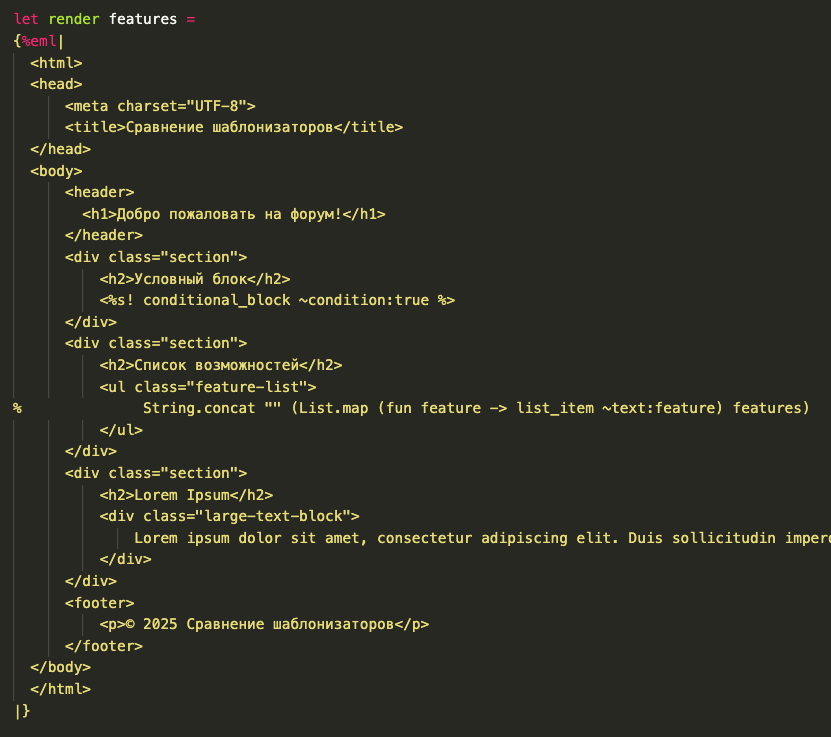
\includegraphics[width=.48\textwidth]{without_highlight}\hfill
    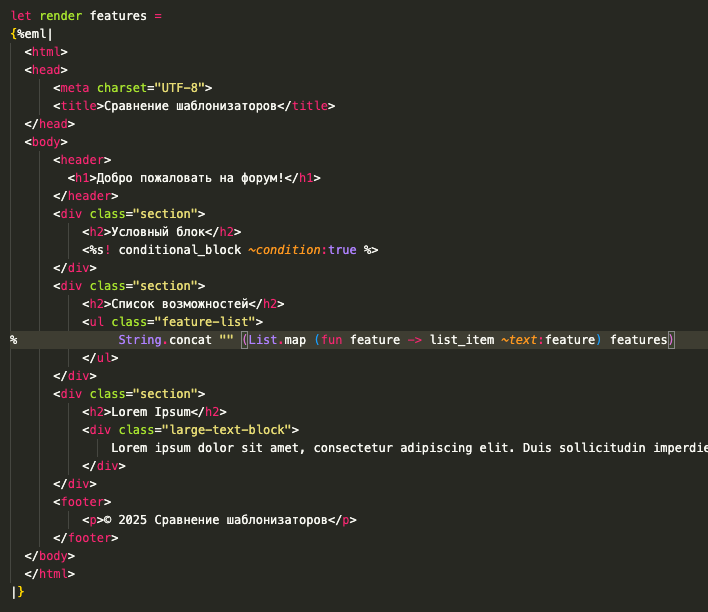
\includegraphics[width=.48\textwidth]{with_highlight}\hfill
    \caption{До изменений, код не подсвечен кроме как строчный литерал}
    \label{fig:without}
    \caption{После изменений, код корректно подсвечен, работают также контекстные подсветки токенов}
    \label{fig:with}
\end{figure}

В VSCode сниппеты настраиваются через JSON-файл, где для каждого шаблона указывается ключевое слово-триггер (prefix), содержимое для вставки (body) и описание.
Пользователь может вызывать сниппеты по соответствующим ключам, ускоряя набор кода и снижая вероятность синтаксических ошибок.
Для каждого языка или шаблонизатора возможно создание собственного набора сниппетов, что существенно облегчает освоение новых инструментов и поддерживает единый стиль кодирования в команде.

Таким образом, реализация расширений для подсветки и сниппетов в VSCode заключается в создании конфигурационных файлов с грамматиками и шаблонами для интересующего языка или DSL и их интеграции в редактор посредством собственных или сторонних расширений.
Для экосистемы OCaml и соответствующих шаблонизаторов такие расширения позволяют повысить удобство работы и ускорить разработку, предоставляя современные инструменты анализа и автодополнения кода прямо в процессе написания приложений на OCaml.

\subsection{Покрытие}

В результатах сравнения было выяснено что EML имеет плохую читабельность генерируемого кода.
В частности, результат получается нечитабельным, поскольку появляется внутреннее представление фреймворка, которое не является частью исходного кода.
Это внутреннее представление, однако, позволяет построить покрытие в целом и явно подсветить строки где код не покрыт.
Например, как видно на \ref{fig:improv_before}.
В связи с этим, было принято решение не изменять эту функциональность, потому что тогда сохранится корректность покрытия.

Рассматривался также вариант добавления указателей для bisect\_ppx, которые экранировали бы сгенерированный EML код.
Однако, этот подход был исключен из рассмотрения по следующим причинам:
bisect\_ppx не предоставляет возможности для экранирования часть кода;
результирующий код все еще должен быть компилируемым OCaml;
метки также должны быть поддержаны в LSP;
Универсального способа, удовлетворяющего всем трем условиям не существует.

Другая проблема заключается в том что весь HTML код шаблона сжимается в 1 строчку с экранированными символами.
Эту проблему можно решить, если использовать встроенный в OCaml\footnote{А также в Reason} синтаскис для многострочных строк.

Старая реализация опиралась на функцию \lstinline{Printf.kprintf} с модификатором \lstinline{%S}, которая экранирует символы и выводит их в генерируемый файл.
Вместо нее, в генерируемый файл будет выводиться строка как есть, заключенная в именованные кавычки
\lstinline{{___eml_tag|}
Имя кавычки необходимо в связи с ограничением синтаксиса многострочных литералов - текст внутри не может содержать последовательность символов |<tag>\}.

С этой проблемой можно было справиться другим способом - проверять код шаблона на наличие такой последовательности и экранировать ее в таком случае.
Однако это решение не является оптимальным, поскольку оно требует дополнительной проверки кода шаблона, а также сильно усложняет код парсера.
Потому более простое решение было выбрано.
Результат этой доработки можно посмотреть на рис. \ref{fig:improv_after}.

\begin{figure}[h!]
    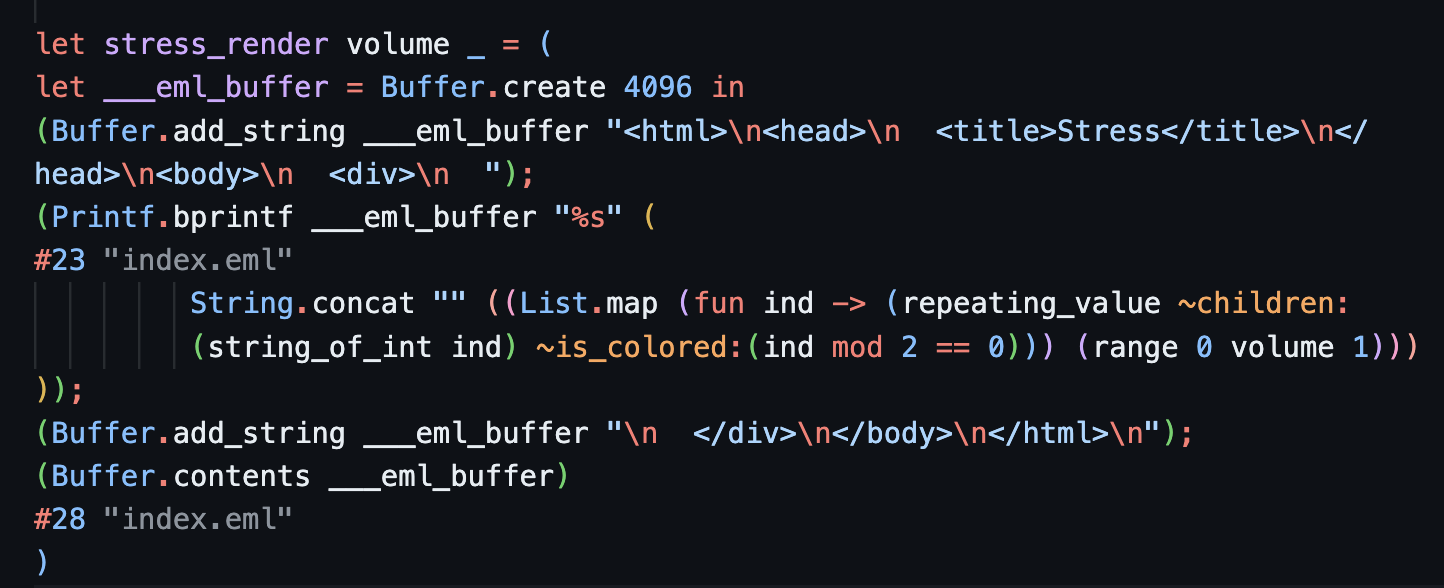
\includegraphics[width=.6\textwidth]{before}\hfill
    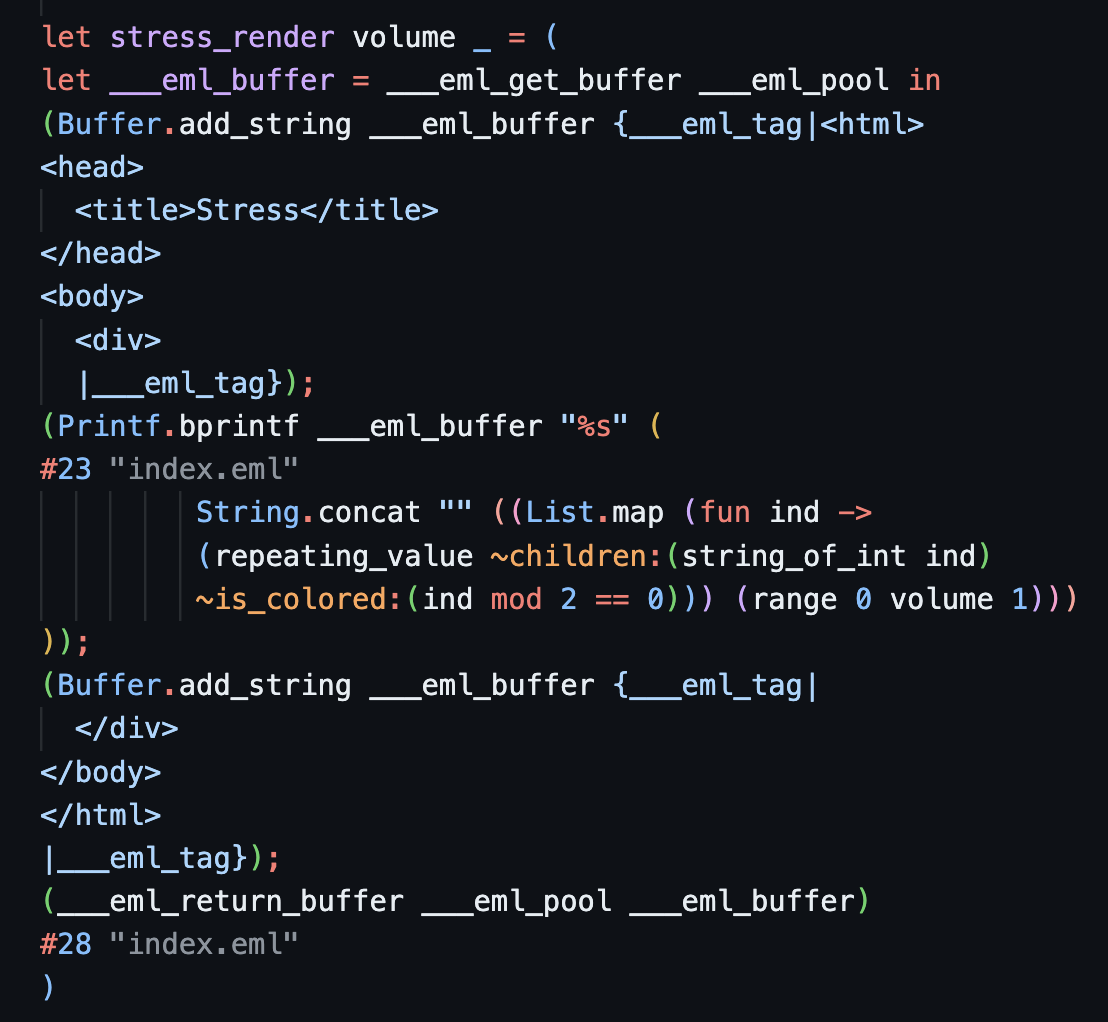
\includegraphics[width=.35\textwidth]{after}\hfill
    \caption{До изменений, код сжат в одну строчку}
    \label{fig:improv_before}
    \caption{После изменений, код раздут в несколько строчек}
    \label{fig:improv_after}
\end{figure}


\subsection{Документация}

Один из критериев оценки был - интеграция с dune.
Dream EML был оценен негативно по этому критерию, так как требует явного указания всех файлов, требующих препроцессинга.
От этого недостатка можно избавиться если воспользоваться встроенной в dune командой для объявления диалекта, подобно MLX %//TODO дока
Реализация приведена на листинге ниже:

\begin{lstlisting}
(dialect
 (name eml)
 (implementation
  (extension eml)
  (preprocess
   (run dream_eml --stdout %{input-file}))))
\end{lstlisting}

Такая реализация позволяет не указывать явно файлы проходящие через препроцессинг, использовать в полнкую силу модульную систему dune, а также использовать расширение .eml для файлов проходящих через препроцессинг.
